% !TeX root = ../thuthesis-example.tex

\chapter{程序设计}

\section{从 C++ 到 Python}

\subsection{包装函数}
一个 Cython 包装函数分为三部分:

\begin{itemize}
    \item 将输入的 Python 对象转换为特定类型的 C++ 变量;
    \item 调用 C/C++ 接口,传入转换后的输入参数;
    \item 将接口的返回值转换为 Python 对象。
\end{itemize}

Cython 能自动处理一部分 C/C++ 类型与 Python 对象间的类型转换,包括基本数值类型、字符串和部分 STL 容器。对于其它类型,包括数组、指针、枚举、类、结构体和联合,CPP2PY 为其专门生成类型转换代码。函数和类方法都以这种方式得到包装。

类的数据成员在 Python 侧被包装为类的属性,CPP2PY 专门为其生成 getter 函数,如果该数据成员或变量是可变的,还会生成 setter 函数。例如,对于如下 C++ 声明,
\begin{framed}
\begin{lstlisting}[language=c++]
struct Point {
    int x;
    const char * LUCKY;
}
\end{lstlisting}
\end{framed}将生成对应 Python 接口,

\begin{framed}
\begin{lstlisting}[language=Python]
class Point:
    @property
    def x(self) -> np.int32: ...
    @x.setter
    def x(self, x: np.int32): ...
    @property
    def LUCKY(self) -> str: ...
\end{lstlisting}
\end{framed}
容易看出,getter 是参数为空,返回值类型为对应变量类型的方法,而 setter 的返回值为空,唯一的参数类型为相应变量类型。生成它们的逻辑与普通的函数或方法完全一致。

CPP2PY 支持 C/C++ 的全局变量,然而,背后的实现机制并不直观。当你在 Python 中写下这段代码时,

\begin{framed}
\begin{lstlisting}[language=python]
pi = 3.14
a = pi
\end{lstlisting}
\end{framed}

\noindent 只有一个对象包含浮点数 3.14,而 \lstinline{a} 和 \lstinline{pi} 都是它的名称。这种赋值机制与 C/C++ 完全不同——对于后者来说,一个变量指向一段内存,赋值表示将数据复制到该内存位置。因此,没有直接的方法将 C 中的变量赋值映射到 Python 中的变量赋值。CPP2PY 处理全局变量的方法是创建一个特殊的全局对象,将全局变量包装为该对象的属性。

这样,CPP2PY 以一种优雅的方式统一封装了变量、函数、方法和数据成员。

\subsection{代理类}

Cython 提供了两种定义类的语法,一种是普通的 Python 类,另一种被称为扩展类。与 Python 类相比,扩展类使用 C 结构体,而不是 Python 字典来存储字段和方法,因而具有显著的性能优势。扩展类中可以存储 C 类型字段,CPP2PY 用它来封装类、结构体与联合。

CPP2PY 在 Cython 端为 C++ 类生成代理类,即同名的 Python 扩展类,其中保存了指向 C++ 对象的指针和标记指针所有权的布尔属性,在构造函数中分配内存并获取所有权,在析构函数中检查所有权、释放内存。代理类机制使得 Python 用户能以非常自然的方式访问 C++ 数据结构。

\begin{framed}
\begin{lstlisting}[language=Python]
def __cinit__(self):
    self.thisptr = NULL
    self.owner = True

def __dealloc__(self):
    if self.owner and self.thisptr != NULL:
        del self.thisptr
        self.thisptr = NULL
\end{lstlisting}
\end{framed}

美中不足的是,与普通 Python 类相比,扩展类只支持有限的面向对象语法。类的静态数据成员不受支持,CPP2PY 将它们视作带作用域的变量;扩展类间的多重继承不受支持,也不允许在子类中重定义 C 类型字段。CPP2PY 以一种间接的方式处理继承——拷贝超类所有的方法和数据成员到派生类中。这种实现的优点是避免生成过于复杂的代码,也支持了多重继承,而缺点则是,类的继承关系将无法从 C++ 映射到 Python 中,第三章中详细阐述了这种妥协带来的限制。

为了计算出一个类所有的超类和派生类,CPP2PY 根据类的继承关系做拓扑排序。

\begin{figure}
  \centering
  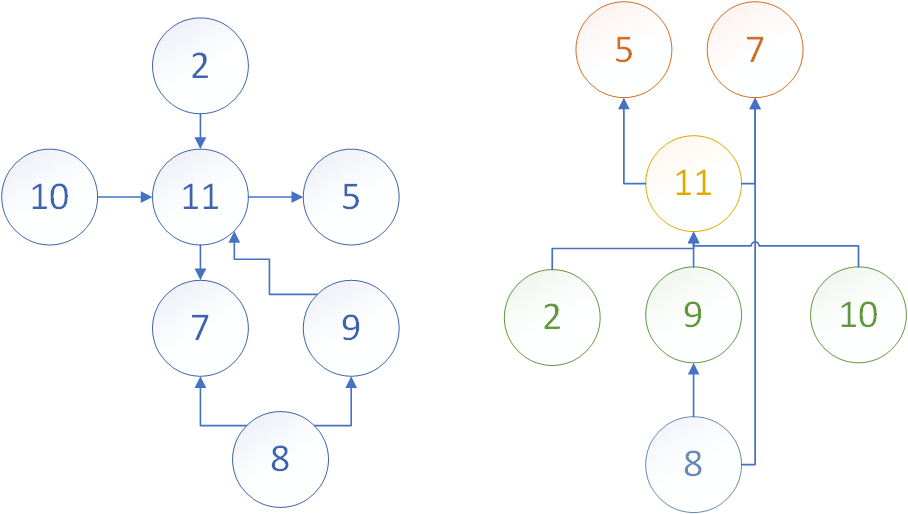
\includegraphics[width=0.8\linewidth]{figures/拓扑排序.png}
  \caption{拓扑排序前后的复杂继承关系图}
  \label{fig:2.4}
\end{figure}

为了说明拓扑排序的效果,考虑如图 \ref{fig:2.4} 左侧所示的复杂继承关系,图中每个节点都代表一个类,每条边由子类指向它的父类,在左图中想要找到类 8 所有的超类并不容易。根据类的父子关系对它们拓扑排序后,得到的结果如图 3 右侧所示。可以立即看出,类 11 依赖于类 5 和类 7,而类 8 依赖于类 9、类11,类 5 和类 7。类 5 和类 7 的拓扑序最靠前,而类 11 次之,类 8 的拓扑序排在最后,一个类的超类在拓扑序列必定排在它前面,派生类必定排在后面。

得到拓扑序后,只需按顺序逐个将每个类的所有父类接口拷贝到类中,即可完成拷贝超类接口的任务。

\section{模块设计}

\begin{figure}
  \centering
  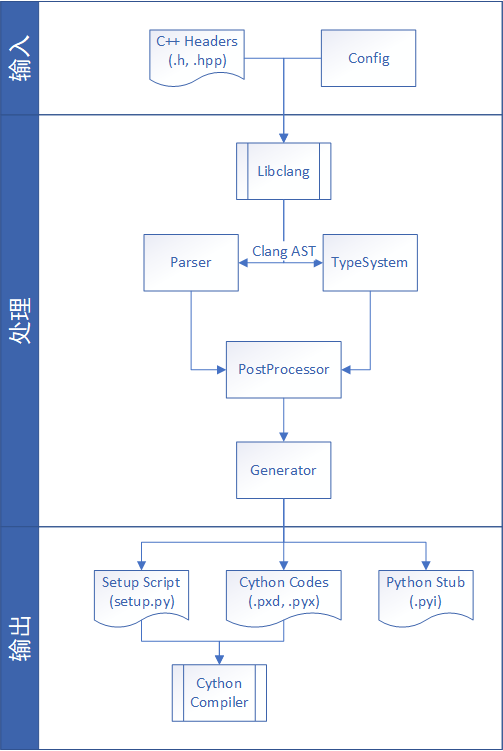
\includegraphics[width=\linewidth]{figures/程序结构.png}
  \caption{模块划分与数据流图}
  \label{fig:2}
\end{figure}

CPP2PY 以 Python 语言编写,其模块设计如图 \ref{fig:2} 所示。程序主要包含五个子模块,分别是 Config、Parser、TypeSystem、PostProcessor 和 Generator;此外还依赖于两个外部库,用于解析 C++ 代码的 libclang 和用于编译目标代码的 Cython。

Config 模块定义了控制程序行为的输入参数,libclang 负责解析 C++ 头文件,生成源文件的抽象语法树 (Abstract Syntax Tree)。Parser 模块解析抽象语法树,从中提取所有必要信息,作为 PostProcessor 的输入。

TypeSystem 建立在 libclang 的类型系统之上。该模块还定义了在 C++ 和 Python 之间转换数据的类型转换器,并对相当一部分类型内置了转换功能。通过继承类型转换器抽象类,用户可以重新定义类型转换的行为,或者使 CPP2PY 支持新的数据类型。

PostProcessor 模块接受 Parser 模块的输入,处理类的继承、函数重载等问题,并为函数、方法和变量绑定类型转换器。

Generator 接受  PostProcessor 的输入,输出目标代码。 生成的文件包括 Cython 代码、Python 构建脚本和存根。

其中, Cython 代码文件分成两部分,所有 C++ 接口的声明在 Cython 声明文件(\lstinline{.pxd})中,而 Cython 实现文件(\lstinline{.pyx})包含了封装这些接口的代码。这样设计使得 C++ 接口与 Python 接口不在同一个作用域内,避免了名称冲突,也给用户二次开发提供了更多的便利。

Python 存根文件与普通 Python 文件的区别是不包含具体实现。利用它,Python IDE 就能为 CPP2PY 生成的二进制代码库提供类型注解和代码补全。得益于此,用户的开发体验将大大提高。不过值得一提的是,作为动态类型语言,Python 并不在乎对象的实际类型,而只关心它是否实现了特定的属性或方法。这种类型系统通常被称为“鸭子类型”。

构建脚本指明了目标代码编译、链接的参数,用户可以根据自己的需要修改构建脚本。虽然 CPP2PY 只在 Ubuntu 上进行了测试,但得益于 Python 构建工具 setuptools,它生成的代码能方便地在不同平台上编译,达到“一次生成,处处构建”的效果。

\section{基于 libclang 的 C++ 头文件解析}

众所周知,C++ 的语法复杂多变,包含了数种编程范式,不计其数的边界情况和庞大的历史包袱。Clang 是 LLVM 的编译前端,支持 C、C++、Objective-C 三种语言的解析。libclang\cite{libclang} 提供了访问 Clang 抽象语法树的 Python 接口,CPP2PY 依赖它完成 C++ 语法解析任务。

Clang 抽象语法树的组成如图 \ref{fig:2.2} 所示,根节点可视为顶层命名空间,它的子节点类型包括命名空间、枚举、类、结构体、联合、变量、函数、类型别名和宏;而类节点的子节点类型又包括数据成员、静态数据成员、方法、构造函数等……根据这样的父子节点关系,Parser 模块层层迭代遍历抽象语法树。

\begin{figure}
  \centering
  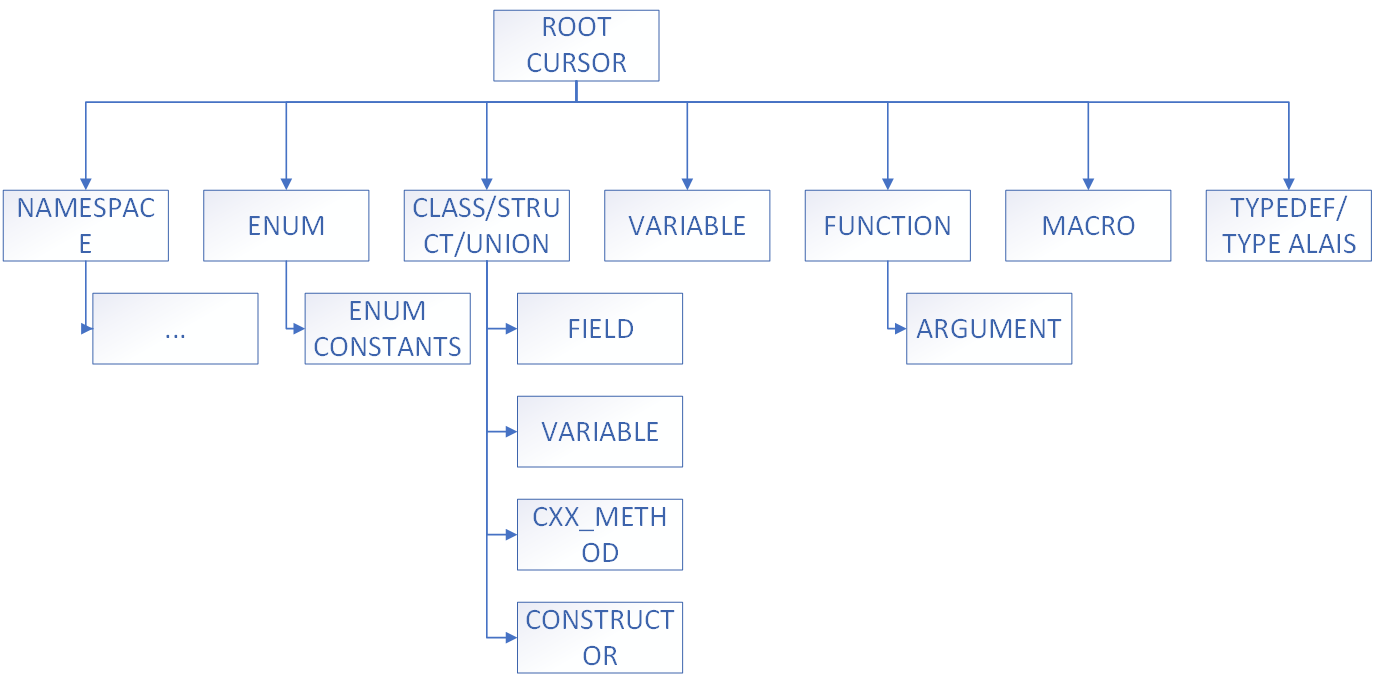
\includegraphics[width=\linewidth]{figures/ClangAST.png}
  \caption{Clang 抽象语法树示意图}
  \label{fig:2.2}
\end{figure}

在解析过程中,C++ 的结构体和联合可以被视作特殊的类,它们的独特之处仅仅在于结构体的成员和继承方式默认为公有,而类默认为私有;联合的所有数据成员共用同一块内存。同样的道理,通过不同语法定义的类型别名也没有实质上的差别。在 C++ 中,通过类的对象访问其非公有成员是不可能的,因此类的任何非公有成员都将被忽略。

解析宏是一件困难的事,因为宏不带有任何额外的类型信息。一个宏可能定义了一段过程、一个类型别名、也可能递归生成了非常复杂的代码。CPP2PY 只能识别定义了简单字面量的宏,包括数值类型和字符串,忽略它解析不了的宏定义。


\section{软件测试}

\begin{figure}
  \centering
  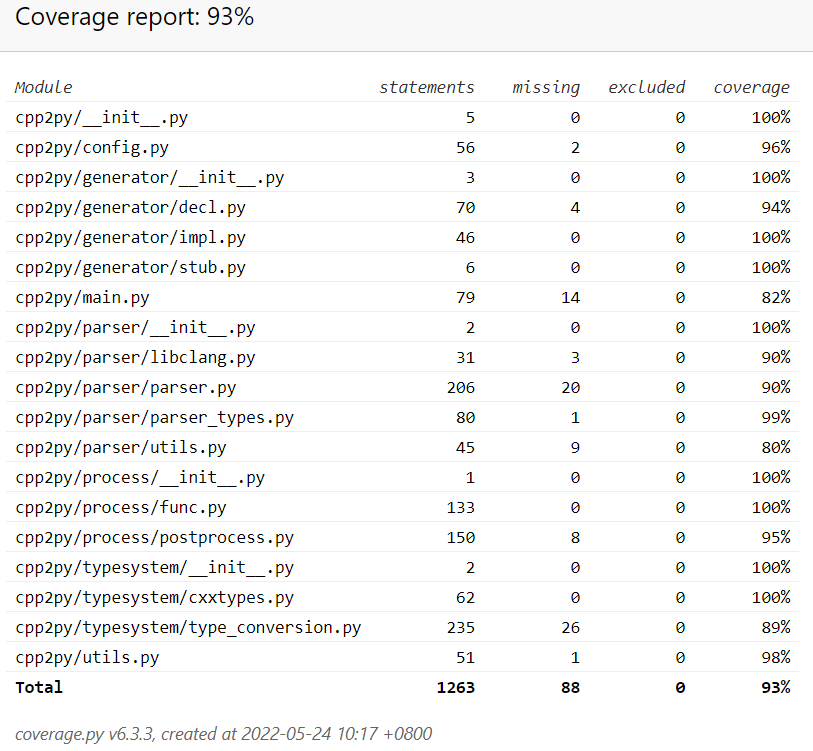
\includegraphics[width=\linewidth]{figures/测试覆盖.png}
  \caption{软件测试覆盖率}
  \label{fig:2.5}
\end{figure}

合理的软件测试既能保证程序的正确运行,又能提高设计和开发的生产力。CPP2PY 的测例分单元测试和集成测试两类。单元测试主要测试程序的功能性模块,如拓扑排序、宏文本解析等。而集成测试以 C++ 代码为输入,测试 CPP2PY 能否正确地解析输入、生成目标代码并编译运行、实现预期的封装效果。

CPP2PY 经过了充分的测试,代码覆盖率达 93\%,如图 \ref{fig:2.5} 所示。测试环境为 Ubuntu 20.04,软件版本为 Python 3.8.10、Cython 0.29.28、libclang 12。
